\documentclass[UTF8]{ctexart}
\hfuzz=4pt

\usepackage{parskip}
    \setlength{\parindent}{0em}
    \setlength{\parskip}{1em}
\usepackage{geometry}
    \geometry{left=4cm,right=4cm,top=2cm,bottom=2cm}
\usepackage{amsmath, amssymb, amsthm, mathtools}
\usepackage{thmtools}
    \renewcommand\qedsymbol{$\blacksquare$}
    \declaretheorem[numberwithin=section,shaded={rulecolor=cyan,rulewidth=2pt,bgcolor=white}]{definition}
    \declaretheorem[numberwithin=section,shaded={rulecolor=orange,rulewidth=2pt, bgcolor=white}]{theorem}
    \newtheoremstyle{mystyle}{1em plus .2 em minus .2em}{1em plus .2 em minus .2em}{}{}{\bfseries}{.}{.5em}{}
    \theoremstyle{mystyle}
    \newtheorem{axiom}{Axiom}[section]
    \newtheorem{lemma}{Lemma}[section]
    \newtheorem{proposition}{Proposition}[section]
    \newtheoremstyle{myremark}{1em plus .2 em minus .2em}{1em plus .2 em minus .2em}{}{}{\itshape}{.}{.5em}{}
    \theoremstyle{myremark}
    \newtheorem*{remark}{Remark}
    \theoremstyle{plain}
    \newtheorem{corollary}{Corollary}[section]
\usepackage{caption}
\usepackage{xcolor}
\usepackage{graphicx}
\usepackage{float}
\usepackage{setspace} 	 % 行间距 \begin{spacing}{arg}
\usepackage{esint}
\usepackage{hyperref}
    \hypersetup{colorlinks=true,linktoc=all,linkcolor=blue}

\newcommand{\ve}[1]{\boldsymbol{\mathbf{#1}}}
\newcommand{\unit}[1]{\boldsymbol{\mathbf{\hat{#1}}}}
\renewcommand{\r}{\mathrm}
\renewcommand{\cal}{\mathcal}
\newcommand{\scr}{\mathscr}

\newcommand{\E}{\mathrm e}
\renewcommand{\I}{\mathrm i}
\newcommand{\R}{\mathbb R}
\newcommand{\Z}{\mathbb Z}
\newcommand{\N}{\mathbb N}
\newcommand{\Q}{\mathbb Q}
\renewcommand{\C}{\mathbb C}
\DeclarePairedDelimiter\set{\{}{\}}
\newcommand{\del}{\nabla}

\pagestyle{empty}

\begin{document}
\section{图与子图}

图有两种定义方式, 一个为二元组, 一个为三元组.

\begin{definition}[\text{图}]
    图 $ G $ 为一个三元组 $ G \coloneqq (V, E, \psi) $, $ V $ 为顶点的集合, $ E $ 为边的集合, $ \psi $ 为边和顶点对的对应关系. 若隐式地的定义边和顶点对的对应关系, 则可以定义 $ G \coloneqq (V, E) $. 对于给定的图 $ G $, 可以记 $ V(G) $, $ E(G) $ 分别代表 $ G $ 的顶点和边集.
\end{definition}

\begin{figure}[H]
    \centering
    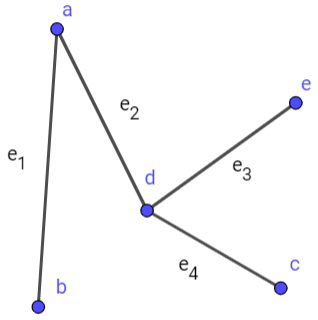
\includegraphics[width = 0.35\linewidth]{./images/graph_definition.png}
    \caption{图 $ G = (V, E, \psi) $}
\end{figure}

\paragraph{例}
上图 $ G $, 其顶点集 $ V = \set{a, b, c, d, e} $, 边集 $ E = \set{e_1, e_2, e_3, e_4} $. 而边和点之间的对应关系为:
\[ \begin{array}{c}
    \psi(e_1) = (a, b) \,,\\
    \psi(e_2) = (a, d) \,,\\
    \psi(e_3) = (d, e) \,,\\
    \psi(e_4) = (d, c)
\end{array} \,.\]





\end{document}